\label{benchmarks}

In this chapter we will benchmark all the categories we explored in
the previous chapter against their default Scala counterparts. We choose a few
representative collections for each category in order to see how the different
transformation strategies and the different collections characteristics affect
the speedups.

\section{Setup}

We used the ScalaMeter~\cite{axel22:scalameter} microbenchmarking and performance regression
testing framework for the JVM platform. We use the same benchmark template for
all the different categories. In short, each benchmark compares the \texttt{macroMap}'s speed against \texttt{map}'s speed
on different sizes of the same collection applying the same closure, the
successor function.

The benchmarks run on a Linux 64-bit machine with an Intel Core i7-2720QM 8-core
CPU and 8GB RAM.

In order to make the benchmarking process more stable, reproducible and reliable
we have tweaked the benchmark template with the following parameters:

\begin{itemize}
 \item 
  each measurement of \texttt{map}/\texttt{macroMap} on a specific collection size is run 25
times successively
 \item
  the 25 measurements are divided on 5 separate JVM instances
 \item
  every 2 measurements the current collection is re-instantiated
 \item
  every 2 measurements a full GC cycle is forced
\end{itemize}


\section{Evaluation}

In Figure~\ref{fig:mut_ind_benchs} we see the benchmark results for \sv{scala.\allowbreak{}collection.\allowbreak{}mutable.\allowbreak{}ArraySeq} 
and \texttt{Array}, as representatives of the mutable indexed
sequences category, i.e., subtypes of \sv{scala.\allowbreak{}collection.\allowbreak{}mutable.\allowbreak{}IndexedSeq} and
\texttt{Array}, where we achieve average speedups of $55\%$ and $88\%$, respectively.

\begin{figure}
  \centering
  \subfloat[\sv{mutable.ArraySeq}~benchmark]{
    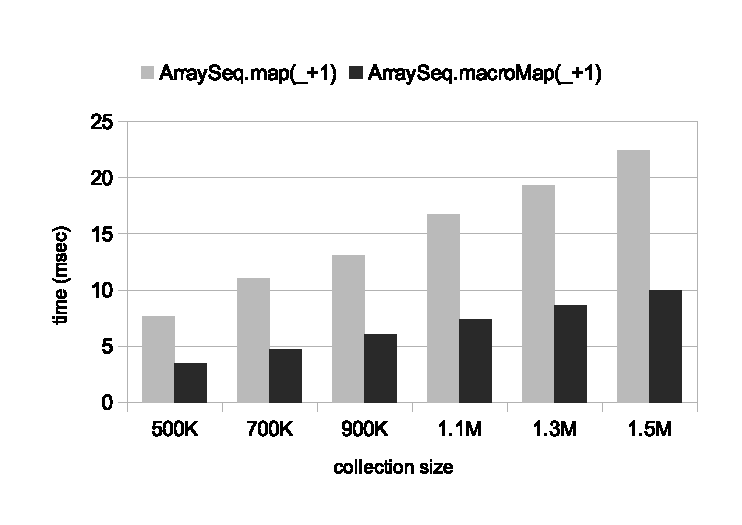
\includegraphics[scale=0.7]{figures/arrayseq_bench.eps}
    \label{fig:arrayseq_bench}
  }
  \subfloat[\texttt{Array}~benchmark]{
    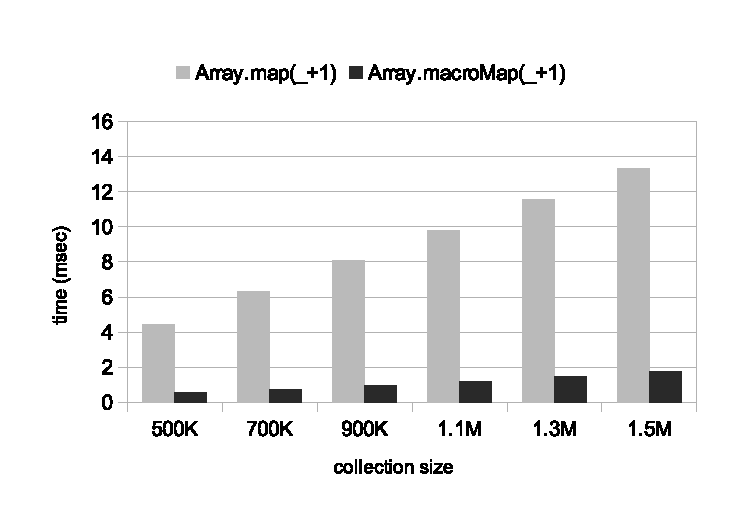
\includegraphics[scale=0.7]{figures/array_bench.eps}
    \label{fig:array_bench}
  }
  \caption{%
    Benchmarks of mutable indexed sequences representatives
  }
\label{fig:mut_ind_benchs}
\end{figure}


The speedup on \texttt{Array} is impressive and the highest one among all the other
benchmarked collections. In this series of benchmarks, all collections hold
integers and the supplied closure returns an integer too (the successor
integer). The Scala language has only one integer type, \sv{scala.Int}, which is similar to Java's
boxed \sv{java.lang.Integer}. scalac tries to use Java's respective primitive types
under the hood, whenever possible, for optimization reasons. More specifically,
after scalac's erasure phase, a \sv{scala.Int} will become either a \texttt{int} or a
\sv{java.lang.Integer}. For example, in our benchmarks, the closure function will
become a local method like:

\begin{scalaCode}
def local1$1(x$1: int): int = x$1.+(1);
\end{scalaCode}

This method deals solely with Java's primitive integers under the hood. On the
other hand, operations on \texttt{ArraySeq}, \texttt{List} and most of the collections except
\texttt{Array}, deal with \sv{java.lang.Integer}. So, for example, in an \texttt{ArraySeq}
transformation the target collection is constructed like this:

\begin{scalaCode}
buf.update(i, scala.Int.box(local1$1(scala.Int.unbox(xs.apply(i))
\end{scalaCode}

while on \texttt{Array}s we have:

\begin{scalaCode}
buf.update(i, local1$1(xs.apply(i)))
\end{scalaCode}

This is due the way \texttt{Array}s are constructed. In particular, when we ask for an
\sv{Array[scala.Int]} in Scala, the compiler inspects it and creates an
\sv{Array[int]} automatically and, as a consequence, all of its methods operate upon
primitive integers. We can see that avoiding the boxing/unboxing operations can
give us a huge performance boost. For that reason, Scala already provides the
\texttt{@specialized} annotation for creating specialized classes/collections and,
more generally, specialization is a hot research topic in the Scala community~\cite{dragos2010compiling,ureche2013miniboxing}.

% Array
% 
% ::Benchmark Array.macroMap::
% Parameters(size -> 500000): 0.56097312
% Parameters(size -> 700000): 0.7099738800000001
% Parameters(size -> 900000): 0.9576477599999998
% Parameters(size -> 1100000): 1.21228168
% Parameters(size -> 1300000): 1.4722931200000002
% Parameters(size -> 1500000): 1.7399196000000001
% 
% ::Benchmark Array.map::
% Parameters(size -> 500000): 4.45799216
% Parameters(size -> 700000): 6.299174839999998
% Parameters(size -> 900000): 8.08378432
% Parameters(size -> 1100000): 9.788586
% Parameters(size -> 1300000): 11.55207984
% Parameters(size -> 1500000): 13.33556824
% 
% 
% ArraySeq
% 
% ::Benchmark ArraySeq.macroMap::
% Parameters(size -> 500000): 3.4582486400000003
% Parameters(size -> 700000): 4.749739399999998
% Parameters(size -> 900000): 6.064567839999999
% Parameters(size -> 1100000): 7.423919880000001
% Parameters(size -> 1300000): 8.668609240000002
% Parameters(size -> 1500000): 9.92232472
% 
% ::Benchmark ArraySeq.map::
% Parameters(size -> 500000): 7.631767120000001
% Parameters(size -> 700000): 11.0168042
% Parameters(size -> 900000): 13.058838600000001
% Parameters(size -> 1100000): 16.710358120000002
% Parameters(size -> 1300000): 19.27880912
% Parameters(size -> 1500000): 22.4225422


In Figure~\ref{fig:lin_bench} we see the benchmark results for \sv{scala.collection.immutable.List},
representative of the linear sequences category, i.e., subtypes of \sv{scala.\allowbreak{}collection.\allowbreak{}LinearSeq}, where we achieve an average speedup of $28\%$.

\begin{figure}
\centering
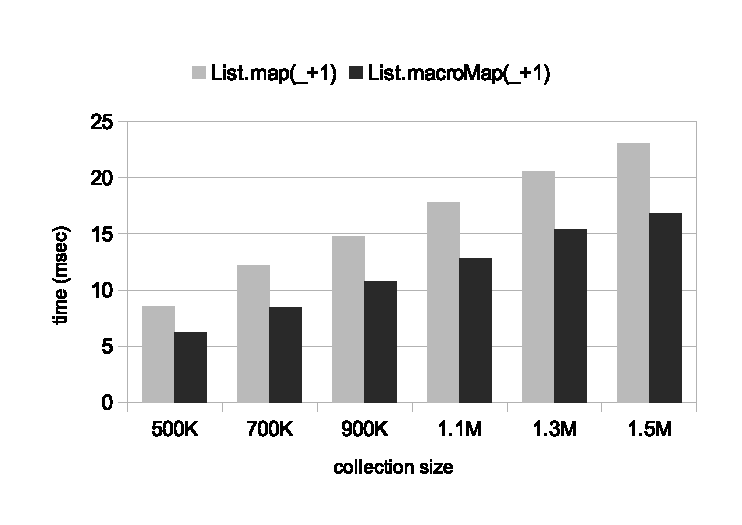
\includegraphics[scale=0.7]{figures/list_bench.eps}
\caption[\texttt{List} benchmark]{\texttt{List} benchmark}
\label{fig:lin_bench}
\end{figure}

% List
% 
% ::Benchmark List.macroMap::
% Parameters(size -> 500000): 6.2594368
% Parameters(size -> 700000): 8.48611428
% Parameters(size -> 900000): 10.796582320000002
% Parameters(size -> 1100000): 12.769916
% Parameters(size -> 1300000): 15.4103694
% Parameters(size -> 1500000): 16.79051676
% 
% ::Benchmark List.map::
% Parameters(size -> 500000): 8.491728160000001
% Parameters(size -> 700000): 12.166298400000002
% Parameters(size -> 900000): 14.759927480000002
% Parameters(size -> 1100000): 17.83202016
% Parameters(size -> 1300000): 20.578929839999997
% Parameters(size -> 1500000): 23.08220884


In Figure~\ref{fig:trav_benchs}, we see the benchmark results for
\sv{scala.\allowbreak{}collection.\allowbreak{}immutable.\allowbreak{}Set} and \sv{scala.\allowbreak{}collection.\allowbreak{}immutable.\allowbreak{}Vector},
representatives of the general category of traversables, i.e., subtypes of \texttt{Traversable}, where we achieve average speedups of $5\%$ and $25\%$, respectively.

Finally, Table~\ref{all_bench_speedups} includes all benchmarks' exact times and their associated speedups.

\begin{figure}
  \centering
  \subfloat[\sv{immutable.Set}~benchmark]{
    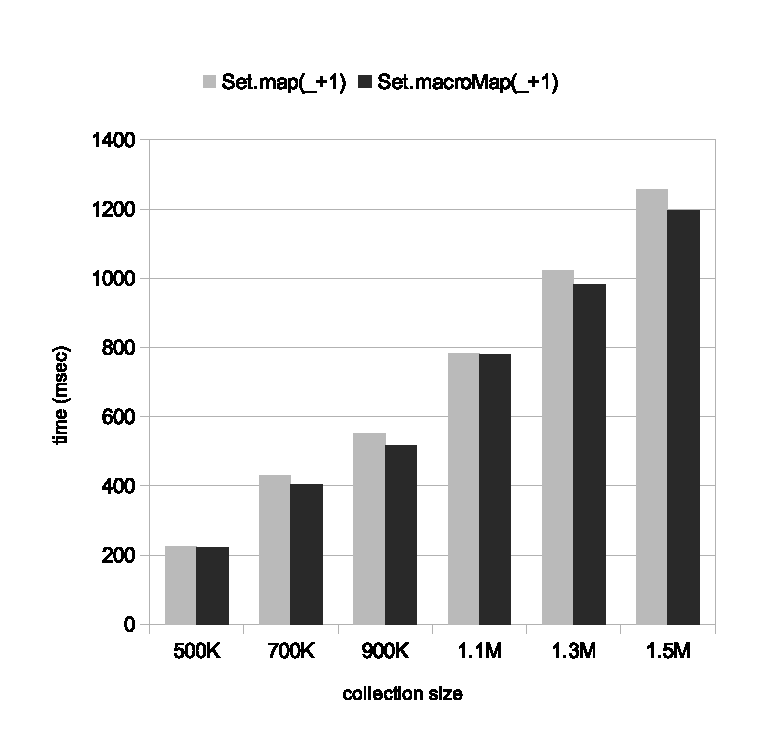
\includegraphics[scale=0.7]{figures/set_bench.eps}
    \label{fig:set_bench}
  }
  \subfloat[\sv{immutable.Vector}~benchmark]{
    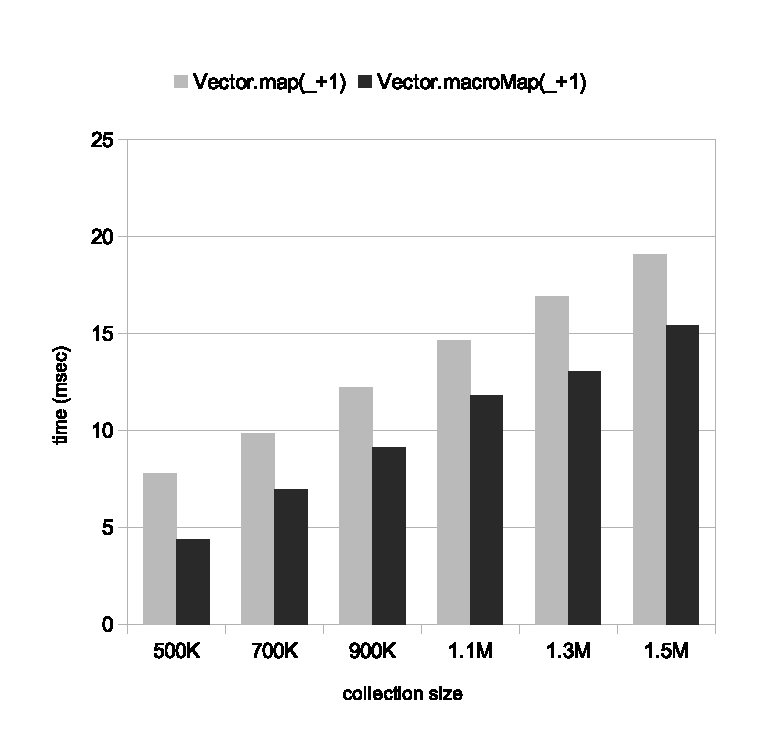
\includegraphics[scale=0.7]{figures/vector_bench.eps}
    \label{fig:vector_bench}
  }
  \caption{%
    Benchmarks of \texttt{Traversable} representatives
  }
\label{fig:trav_benchs}
\end{figure}


% Set
% 
% ::Benchmark Set.macroMap::
% Parameters(size -> 500000): 221.49879935999996
% Parameters(size -> 700000): 404.7653434
% Parameters(size -> 900000): 517.1970278800001
% Parameters(size -> 1100000): 780.3368136800001
% Parameters(size -> 1300000): 980.5737080400002
% Parameters(size -> 1500000): 1196.13017984
% 
% ::Benchmark Set.map::
% Parameters(size -> 500000): 225.10970228
% Parameters(size -> 700000): 428.7541246000001
% Parameters(size -> 900000): 552.35796532
% Parameters(size -> 1100000): 783.1912343599998
% Parameters(size -> 1300000): 1021.149488
% Parameters(size -> 1500000): 1256.03854812
% 
% 
% Vector
% ::Benchmark Vector.macroMap::
% Parameters(size -> 500000): 4.3560588000000005
% Parameters(size -> 700000): 6.97072312
% Parameters(size -> 900000): 9.13849436
% Parameters(size -> 1100000): 11.800523919999998
% Parameters(size -> 1300000): 13.052000560000003
% Parameters(size -> 1500000): 15.433811600000002
% 
% ::Benchmark Vector.map::
% Parameters(size -> 500000): 7.798935959999999
% Parameters(size -> 700000): 9.82132696
% Parameters(size -> 900000): 12.20604608
% Parameters(size -> 1100000): 14.643066959999999
% Parameters(size -> 1300000): 16.92755692
% Parameters(size -> 1500000): 19.05916

\begin{table}
\centering
\scalebox{0.8}{
\begin{tabular} {|c|c|l|r|r|r|r|r|r|}
\cline{4-9}
\multicolumn{3}{c}{} & \multicolumn{6}{|c|}{Collection Sizes}\\
\hline
Transformation Category & Collection & Method & 500K & 700K & 900K & 1.1M & 1.3M & 1.5M\\
\hline
% \multirow{6}{*}{\rotatebox{90}{mut. ind. seq. }}
\multirow{6}{*}{Mutable Indexed Seq.}
& \multirow{3}{*}{ArraySeq} & map & $07.63$ & $11.02$ & $13.06$ & $16.71$ & $19.28$ & $22.42$\\
\cline{3-9}
& & macroMap & $03.46$ & $04.75$ & $06.06$ & $07.42$ & $08.67$ & $09.92$\\
\cline{3-9}
& & \emph{speedup} & $54.65\%$ & $56.89\%$ & $53.59\%$ & $55.59\%$ & $55.03\%$ & $55.75\%$\\
\cline{2-9}

& \multirow{3}{*}{Array} & map & $04.46$ & $06.30$ & $08.08$ & $09. 79$ & $11.55$ & $13.34$\\
\cline{3-9}
& & macroMap & $00.56$ & $00.71$ & $00.96$ & $01.21$ & $01.47$ & $01.74$\\
\cline{3-9}
& & \emph{speedup} & $87.44\%$ & $88.73\%$ & $88.11\%$ & $87.64\%$ & $87.27\%$ & $86.95\%$\\
\hline

\multirow{3}{*}{Linear Seq.}
& \multirow{3}{*}{List} & map & $08.49$ & $12.17$ & $14.76$ & $17.83$ & $20.58$ & $23.08$\\
\cline{3-9}
& & macroMap & $06.26$ & $08.49$ & $10.80$ & $12.77$ & $15.41$ & $16.79$\\
\cline{3-9}
& & \emph{speedup} & $26.27\%$ & $30.24\%$ & $26.83\%$ & $28.37\%$ & $25.12\%$ & $27.25\%$\\
\hline

\multirow{6}{*}{Traversable}
& \multirow{3}{*}{Set} & map & $225.10$ & $428.75$ & $552.36$ & $783.19$ & $1021.15$ & $1256.04$\\
\cline{3-9}
& & macroMap & $221.50$ & $404.77$ & $517.20$ & $780.34$ & $980.57$ & $1196.13$\\
\cline{3-9}
& & \emph{speedup} & $01.60\%$ & $05.60\%$ & $06.37\%$ & $00.36\%$ & $03.40\%$ & $04.77\%$\\
\cline{2-9}

& \multirow{3}{*}{Vector} & map & $07.80$ & $09.82$ & $12.20$ & $14.64$ & $16.93$ & $19.06$\\
\cline{3-9}
& & macroMap & $04.35$ & $06.97$ & $09.13$ & $11.80$ & $13.05$ & $15.43$\\
\cline{3-9}
& & \emph{speedup} & $44.23\%$ & $29.02\%$ & $25.16\%$ & $19.39\%$ & $22.92\%$ & $19.05\%$\\
\hline

\end{tabular}
}
\caption[Collections Benchmarks and Speedups]{Collections Benchmarks and Speedups}
\label{all_bench_speedups}
\end{table}
